% questions.tex —— 2022 年·全国甲卷·文科 · 题目内容片段（无答案）
% 由 tools/generate_projects.py 依来源总账自 2022/2022_数学真题_全国甲文_试题.md 生成，勿手改（改源 MD 后重跑）


\gkpart{一、单选题}

\begin{question}
\gkti{1}设集合 $A=\{-2,-1,0,1,2\}$，$B=\{x\mid 0\leq x<\dfrac52\}$，则 $A\cap B=$\mbox{（　　）}

\begin{gkopts}(4)
\task A．$\{0,1,2\}$
\task B．$\{-2,-1,0\}$
\task C．$\{0,1\}$
\task D．$\{1,2\}$
\end{gkopts}

\Needspace{0.4\textheight}
\end{question}
\begin{question}
\gkti{2}某社区通过公益讲座以普及社区居民的垃圾分类知识。为了解讲座效果，随机抽取 10 位社区居民，让他们在讲座前和讲座后各回答一份垃圾分类知识问卷，这 10 位社区居民在讲座前和讲座后问卷答题的正确率如下图：

图中 \textbullet{} 表示讲座后，＊表示讲座前；散点图见下图。
\nopagebreak[4]
\begin{center}\begin{tikzpicture}[x=0.58cm,y=0.09cm,font=\small]
  % PDF p.1，纸面 p.1163；纵轴在 60 处断轴。
  \draw (0,0) -- (0,55);
  \draw[->] (0,60) -- (0,105) node[above] {正确率};
  \draw[->] (0,0) -- (12.8,0) node[right] {居民编号};
  \draw (-0.12,55) -- (0.12,57) -- (-0.12,59);
  \foreach \y in {60,65,70,75,80,85,90,95,100} {
    \draw[gray!55] (0,\y) -- (10,\y);
    \node[left] at (0,\y) {\y};
  }
  \foreach \x in {1,...,10} {
    \draw (\x,0) -- (\x,2);
    \node[below] at (\x,0) {\x};
  }
  \foreach \x/\y in {1/90,2/85,3/80,4/90,5/85,6/85,7/95,8/100,9/85,10/100} {
    \fill (\x,\y) circle (1.8pt);
  }
  \foreach \x/\y in {1/65,2/60,3/70,4/60,5/65,6/75,7/90,8/85,9/80,10/95} {
    \node[inner sep=0pt] at (\x,\y) {$\ast$};
  }
  \fill (11.1,92) circle (1.8pt);
  \node[anchor=west] at (11.4,92) {讲座后};
  \node[anchor=west] at (11.1,86) {$\ast$ 讲座前};
\end{tikzpicture}
\end{center}
\nopagebreak[4]
则\mbox{（　　）}

\begin{gkopts}(1)
\task A．讲座前问卷答题的正确率的中位数小于 $70\%$
\task B．讲座后问卷答题的正确率的平均数大于 $85\%$
\task C．讲座前问卷答题的正确率的标准差小于讲座后正确率的标准差
\task D．讲座后问卷答题的正确率的极差大于讲座前正确率的极差
\end{gkopts}

\end{question}
\begin{question}
\gkti{3}若 $z=1+\mathrm i$，则 $\left|\mathrm iz+3\bar z\right|=$\mbox{（　　）}

\begin{gkopts}(4)
\task A．$4\sqrt5$
\task B．$4\sqrt2$
\task C．$2\sqrt5$
\task D．$2\sqrt2$
\end{gkopts}

\Needspace{0.4\textheight}
\end{question}
\begin{question}
\gkti{4}如图，网格纸上绘制的是一个多面体的三视图，网格小正方形的边长为 $1$，则该多面体的体积为\mbox{（　　）}

三视图见下图。
\nopagebreak[4]
\begin{center}\begin{tikzpicture}[x=0.42cm,y=0.42cm,font=\small]
  \begin{scope}
    \foreach \x in {0,...,6} \draw[gray!50] (\x,0) -- (\x,4);
    \foreach \y in {0,...,4} \draw[gray!50] (0,\y) -- (6,\y);
    \draw[thick] (1,1) -- (5,1) -- (3,3) -- (1,3) -- cycle;
  \end{scope}
  \begin{scope}[xshift=8cm]
    \foreach \x in {0,...,6} \draw[gray!50] (\x,0) -- (\x,4);
    \foreach \y in {0,...,4} \draw[gray!50] (0,\y) -- (6,\y);
    \draw[thick] (2,1) rectangle (4,3);
  \end{scope}
  \begin{scope}[yshift=-5cm]
    \foreach \x in {0,...,6} \draw[gray!50] (\x,0) -- (\x,4);
    \foreach \y in {0,...,4} \draw[gray!50] (0,\y) -- (6,\y);
    \draw[thick] (1,1) rectangle (5,3);
    \draw[thick] (3,1) -- (3,3);
  \end{scope}
\end{tikzpicture}
\end{center}
\nopagebreak[4]
\begin{gkopts}(4)
\task A．$8$
\task B．$12$
\task C．$16$
\task D．$20$
\end{gkopts}

\end{question}
\begin{question}
\gkti{5}将函数 $f(x)=\sin\left(\omega x+\dfrac{\pi}{3}\right)\ (\omega>0)$ 的图象向左平移 $\dfrac{\pi}{2}$ 个单位长度后得到曲线 $C$，若 $C$ 关于 $y$ 轴对称，则 $\omega$ 的最小值为\mbox{（　　）}

\begin{gkopts}(4)
\task A．$\dfrac16$
\task B．$\dfrac14$
\task C．$\dfrac13$
\task D．$\dfrac12$
\end{gkopts}

\end{question}
\begin{question}
\gkti{6}从分别写有 $1,2,3,4,5,6$ 的 6 张卡片中无放回随机抽取 2 张，则抽到的 2 张卡片上的数字之积是 4 的倍数的概率为\mbox{（　　）}

\begin{gkopts}(4)
\task A．$\dfrac15$
\task B．$\dfrac13$
\task C．$\dfrac25$
\task D．$\dfrac23$
\end{gkopts}

\Needspace{0.4\textheight}
\end{question}
\begin{question}
\gkti{7}函数 $y=(3^x-3^{-x})\cos x$ 在区间 $\left[-\dfrac{\pi}{2},\dfrac{\pi}{2}\right]$ 的图象大致为\mbox{（　　）}

四个候选曲线见下图。
\nopagebreak[4]
\begin{center}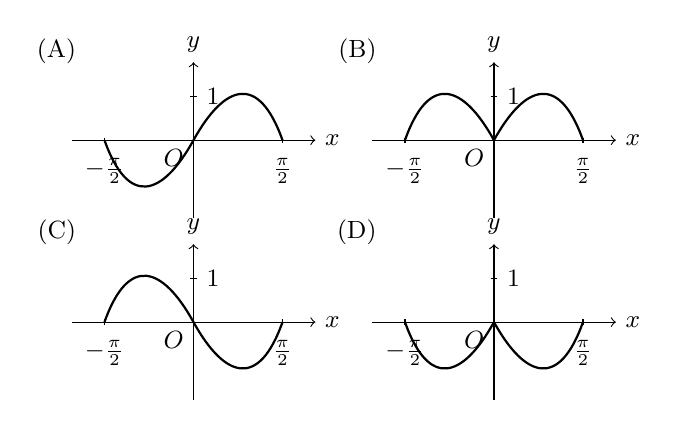
\begin{tikzpicture}[x=0.72cm,y=0.55cm,font=\small]
  \foreach \x/\y/\lab in {0/0/A,5.3/0/B,0/-4.2/C,5.3/-4.2/D} {
    \begin{scope}[shift={(\x,\y)}]
      \draw[->] (-2.15,0) -- (2.15,0) node[right] {$x$};
      \draw[->] (0,-1.8) -- (0,1.8) node[above] {$y$};
      \draw (-0.06,1) -- (0.06,1) node[right] {$1$};
      \draw (-1.57,0.06) -- (-1.57,-0.06) node[below=2pt] {$-\frac{\pi}{2}$};
      \draw (1.57,0.06) -- (1.57,-0.06) node[below=2pt] {$\frac{\pi}{2}$};
      \node[below left] at (0,0) {$O$};
      \node[above left] at (-1.9,1.55) {(\lab)};
    \end{scope}
  }
  \draw[thick] (-1.57,0) .. controls (-1.15,-1.55) and (-0.55,-1.3) .. (0,0)
               .. controls (0.55,1.3) and (1.15,1.55) .. (1.57,0);
  \draw[thick] (5.3-1.57,0) .. controls (5.3-1.15,1.55) and (5.3-0.55,1.3) .. (5.3,0)
               .. controls (5.3+0.55,1.3) and (5.3+1.15,1.55) .. (5.3+1.57,0);
  \draw[thick] (-1.57,-4.2) .. controls (-1.15,-4.2+1.55) and (-0.55,-4.2+1.3) .. (0,-4.2)
               .. controls (0.55,-4.2-1.3) and (1.15,-4.2-1.55) .. (1.57,-4.2);
  \draw[thick] (5.3-1.57,-4.2) .. controls (5.3-1.15,-4.2-1.55) and (5.3-0.55,-4.2-1.3) .. (5.3,-4.2)
               .. controls (5.3+0.55,-4.2-1.3) and (5.3+1.15,-4.2-1.55) .. (5.3+1.57,-4.2);
\end{tikzpicture}
\end{center}
\nopagebreak[4]
\end{question}
\begin{question}
\gkti{8}当 $x=1$ 时，函数 $f(x)=a\ln x+\dfrac bx$ 取得最大值 $-2$，则 $f'(2)=$\mbox{（　　）}

\begin{gkopts}(4)
\task A．$-1$
\task B．$-\dfrac12$
\task C．$\dfrac12$
\task D．$1$
\end{gkopts}

\end{question}
\begin{question}
\gkti{9}在长方体 $ABCD-A_1B_1C_1D_1$ 中，已知 $B_1D$ 与平面 $ABCD$ 和平面 $AA_1B_1B$ 所成的角均为 $30^\circ$，则\mbox{（　　）}

\begin{gkopts}(1)
\task A．$AB=2AD$
\task B．$AB$ 与平面 $AB_1C_1D$ 所成的角为 $30^\circ$
\task C．$AC=CB_1$
\task D．$B_1D$ 与平面 $BB_1C_1C$ 所成的角为 $45^\circ$
\end{gkopts}

\end{question}
\begin{question}
\gkti{10}甲、乙两个圆锥的母线长相等，侧面展开图的圆心角之和为 $2\pi$，侧面积分别为 $S_{\text{\text{甲}}}$ 和 $S_{\text{\text{乙}}}$，体积分别为 $V_{\text{\text{甲}}}$ 和 $V_{\text{\text{乙}}}$。若 $\dfrac{S_{\text{\text{甲}}}}{S_{\text{\text{乙}}}}=2$，则 $\dfrac{V_{\text{\text{甲}}}}{V_{\text{\text{乙}}}}=$\mbox{（　　）}

\begin{gkopts}(2)
\task A．$\sqrt5$
\task B．$2\sqrt2$
\task C．$\sqrt{10}$
\task D．$\dfrac{5\sqrt{10}}4$
\end{gkopts}

\end{question}
\begin{question}
\gkti{11}已知椭圆 $C:\dfrac{x^2}{a^2}+\dfrac{y^2}{b^2}=1\ (a>b>0)$ 的离心率为 $\dfrac13$，$A_1,A_2$ 分别为 $C$ 的左、右顶点，$B$ 为 $C$ 的上顶点。若 $\overrightarrow{BA_1}\cdot\overrightarrow{BA_2}=-1$，则 $C$ 的方程为\mbox{（　　）}

\begin{gkopts}(2)
\task A．$\dfrac{x^2}{18}+\dfrac{y^2}{16}=1$
\task B．$\dfrac{x^2}{9}+\dfrac{y^2}{8}=1$
\task C．$\dfrac{x^2}{3}+\dfrac{y^2}{2}=1$
\task D．$\dfrac{x^2}{2}+y^2=1$
\end{gkopts}

\end{question}
\begin{question}
\gkti{12}已知 $9^m=10$，$a=10^m-11$，$b=8^m-9$，则\mbox{（　　）}

\begin{gkopts}(4)
\task A．$a>0>b$
\task B．$a>b>0$
\task C．$b>a>0$
\task D．$b>0>a$
\end{gkopts}

\end{question}
\gkpart{二、填空题}

\begin{question}
\gkti{13}已知向量 $\boldsymbol a=(m,3)$，$\boldsymbol b=(1,m+1)$。若 $\boldsymbol a\perp\boldsymbol b$，则 $m=$\gkblank{}。

\end{question}
\begin{question}
\gkti{14}设点 $M$ 在直线 $2x+y-1=0$ 上，点 $(3,0)$ 和 $(0,1)$ 均在 $\odot M$ 上，则 $\odot M$ 的方程为\gkblank{}。

\end{question}
\begin{question}
\gkti{15}记双曲线 $C:\dfrac{x^2}{a^2}-\dfrac{y^2}{b^2}=1\ (a>0,b>0)$ 的离心率为 $e$，写出满足条件“直线 $y=2x$ 与 $C$ 无公共点”的 $e$ 的一个值\gkblank{}。

\end{question}
\begin{question}
\gkti{16}已知 $\triangle ABC$ 中，点 $D$ 在边 $BC$ 上，$\angle ADB=120^\circ$，$AD=2$，$CD=2BD$。当 $\dfrac{AC}{AB}$ 取得最小值时，$BD=$\gkblank{}。

\end{question}
\gkpart{三、解答题}

\begin{question}
\gkti{17}甲、乙两城之间的长途客车均由 $A$ 和 $B$ 两家公司运营。为了解这两家公司的长途客车的运行情况，随机调查了甲、乙两城之间的 500 个班次，得到下面列联表：

\begin{center}
\begin{tabular}{lrr}
\toprule
公司 & 准点班次数 & 未准点班次数 \\
\midrule
A & 240 & 20 \\
B & 210 & 30 \\
\bottomrule
\end{tabular}
\end{center}

(1) 根据上表，分别估计这两家公司甲、乙两城之间的长途客车准点的概率；  
(2) 能否有 $90\%$ 的把握认为甲、乙两城之间的长途客车是否准点与客车所属公司有关？

\Needspace{10\baselineskip}
附：$K^2=\dfrac{n(ad-bc)^2}{(a+b)(c+d)(a+c)(b+d)}$，

\begin{center}
\begin{tabular}{lrrr}
\toprule
$P(K^2\geq k)$ & $0.100$ & $0.050$ & $0.010$ \\
\midrule
$k$ & $2.706$ & $3.841$ & $6.635$ \\
\bottomrule
\end{tabular}
\end{center}

\end{question}
\begin{question}
\gkti{18}记 $S_n$ 为数列 $\{a_n\}$ 的前 $n$ 项和。已知
\nopagebreak[4]
\[\frac{2S_n}{n}+n=2a_n+1.\]
(1) 证明：$\{a_n\}$ 是等差数列；  
(2) 若 $a_4,a_7,a_9$ 成等比数列，求 $S_n$ 的最小值。

\Needspace{0.4\textheight}
\end{question}
\begin{question}
\gkti{19}小明同学参见综合实践活动，设计了一个封闭的包装盒。包装盒如图所示：底面 $ABCD$ 是边长为 $8$（单位：cm）的正方形，$\triangle EAB,\triangle FBC,\triangle GCD,\triangle HDA$ 均为正三角形，且它们所在的平面都与平面 $ABCD$ 垂直。

包装盒示意图如下。
\nopagebreak[4]
\begin{center}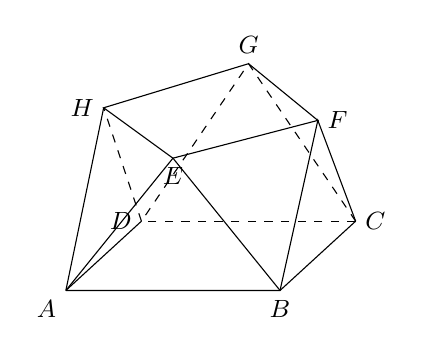
\begin{tikzpicture}[x=0.8cm,y=0.8cm,font=\small]
  \coordinate (A) at (0,0);
  \coordinate (B) at (3.4,0);
  \coordinate (C) at (4.6,1.1);
  \coordinate (D) at (1.2,1.1);
  \coordinate (E) at (1.7,2.1);
  \coordinate (F) at (4.0,2.7);
  \coordinate (G) at (2.9,3.6);
  \coordinate (H) at (0.6,2.9);
  \draw (A)--(B)--(C);
  \draw[dashed] (C)--(D);
  \draw (D)--(A);
  \draw (A)--(E)--(B);
  \draw (B)--(F)--(C);
  \draw[dashed] (C)--(G)--(D);
  \draw[dashed] (D)--(H);
  \draw (H)--(A);
  \draw (E)--(F)--(G);
  \draw (G)--(H)--(E);
  \node[below left] at (A) {$A$};
  \node[below] at (B) {$B$};
  \node[right] at (C) {$C$};
  \node[left] at (D) {$D$};
  \node[below] at (E) {$E$};
  \node[right] at (F) {$F$};
  \node[above] at (G) {$G$};
  \node[left] at (H) {$H$};
\end{tikzpicture}
\end{center}
\nopagebreak[4]
(1) 证明：$EF\parallel$ 平面 $ABCD$；  
(2) 求该包装盒的容积（不计包装盒材料的厚度）。

\end{question}
\begin{question}
\gkti{20}已知函数 $f(x)=x^3-x$，$g(x)=x^2+a$，曲线 $y=f(x)$ 在点 $(x_1,f(x_1))$ 处的切线也是曲线 $y=g(x)$ 的切线。

(1) 若 $x_1=-1$，求 $a$；  
(2) 求 $a$ 的取值范围。

\end{question}
\begin{question}
\gkti{21}设抛物线 $C:y^2=2px\ (p>0)$ 的焦点为 $F$，点 $D(p,0)$，过 $F$ 的直线交 $C$ 于 $M,N$ 两点。当直线 $MD$ 垂直于 $x$ 轴时，$|MF|=3$。

(1) 求 $C$ 的方程；  
(2) 设直线 $MD,ND$ 与 $C$ 的另一个交点分别为 $A,B$，记直线 $MN,AB$ 的倾斜角分别为 $\alpha,\beta$。当 $\alpha-\beta$ 取得最大值时，求直线 $AB$ 的方程。

\end{question}
\begin{question}
\gkti{22}在直角坐标系 $xOy$ 中，曲线 $C_1$ 的参数方程为
\nopagebreak[4]
\[\begin{cases}x=\dfrac{2+t}{6},\\ y=\sqrt t\end{cases}\quad(t\text{ \text{为参数}}),\]
\Needspace{5\baselineskip}
曲线 $C_2$ 的参数方程为
\nopagebreak[4]
\[\begin{cases}x=-\dfrac{2+s}{6},\\ y=-\sqrt s\end{cases}\quad(s\text{ \text{为参数}}).\]
(1) 写出 $C_1$ 的普通方程；  
(2) 以坐标原点为极点，$x$ 轴正半轴为极轴建立极坐标系，曲线 $C_3$ 的极坐标方程为 $2\cos\theta-\sin\theta=0$，求 $C_3$ 与 $C_1$ 交点的直角坐标，及 $C_3$ 与 $C_2$ 交点的直角坐标。

\end{question}
\begin{question}
\gkti{23}已知 $a,b,c$ 均为正数，且 $a^2+b^2+4c^2=3$，证明：

(1) $a+b+2c\leq3$；  
(2) 若 $b=2c$，则 $\dfrac1a+\dfrac1c\geq3$。

\end{question}